\documentclass[11pt]{article}
\usepackage[margin=.7in, top=1in]{geometry}
\usepackage[all]{nowidow}
\usepackage[hyperfigures=true, hidelinks, pdfhighlight=/N]{hyperref}
\usepackage[separate-uncertainty=true, group-digits=false]{siunitx}
\usepackage{graphicx,amsmath,physics,tabto,float,amssymb,pgfplots,verbatim,tcolorbox}
\usepackage{listings,xcolor,subfig,caption,import,wrapfig,biblatex}
\usepackage[version=4]{mhchem}
\usepackage[noabbrev]{cleveref}
\newcommand{\creflastconjunction}{, and\nobreakspace}
\newcommand{\mb}[1]{\mathbf{#1}}
\numberwithin{equation}{section}
\numberwithin{figure}{section}
\numberwithin{table}{section}
\definecolor{stringcolor}{HTML}{C792EA}
\definecolor{codeblue}{HTML}{2162DB}
\definecolor{commentcolor}{HTML}{4A6E46}
\captionsetup{font=small, belowskip=0pt}
\lstdefinestyle{appendix}{
    basicstyle=\ttfamily\footnotesize,commentstyle=\color{commentcolor},keywordstyle=\color{codeblue},
    stringstyle=\color{stringcolor},showstringspaces=false,numbers=left,upquote=true,captionpos=t,
    abovecaptionskip=12pt,belowcaptionskip=12pt,language=Python,breaklines=true,frame=single}
\lstdefinestyle{inline}{
    basicstyle=\ttfamily\footnotesize,commentstyle=\color{commentcolor},keywordstyle=\color{codeblue},
    stringstyle=\color{stringcolor},showstringspaces=false,numbers=left,upquote=true,frame=tb,
    captionpos=b,language=Python}
\renewcommand{\lstlistingname}{Appendix}
\pgfplotsset{compat=1.17}
\addbibresource{bibliography.bib}

\begin{document}

\begin{center}
    {\huge Investigating the first positron detection}\\
    \vspace{0.2in}
    \textbf{KDSMIL001 | August 2022}
    
    \begin{abstract}
        The first image of a positron track in a cloud chamber is analysed in a similar way to the original paper. The momentum of the particle in two regions, as well as mass stopping power for the particle, is found using a graphical method. 
    \end{abstract}
\end{center}

\section{Introduction}\label{sec:Introduction}
The discovery of the electron is credited to J.J. Thomson in 1897, showing that the atom was not the homogeneous, indivisible thing that it had previously been believed to be. By convention of electrical circuits, its charge was given as $-e\approx-\SI{1.602e-19}{\coulomb}$, where we call $e$ the ``fundamental charge''. In 1933, Carl Anderson published a paper called `The Positive Electron'~\cite{Pos_Electron}, in which he showed images of tracks of particles coming from cosmic rays. He claimed that due to their charge to mass ratio as well as their energy-loss, the only option was for them to be a particle of the same mass as an electron, but with opposite charge. He called this the ``positron''. 

This report will recreate the analysis performed by Anderson, acting as if the data taken was our own.

\section{Background}\label{sec:Background}
As charged particles pass through matter, they deposit some energy in the matter. A type of detector called a cloud chamber (or Wilson chamber) was developed that takes advantage of this phenomenon. It consists of a chamber filled with a supersaturated vapour of alcohol or water. As a charged particle travels through the vapour, it ionises some particles, creating nucleation sites for condensation to occur, creating small clouds around the path of the particle. These particle tracks can then be captured by taking a photograph of the chamber.

In order to learn more about the particles being studied, a uniform magnetic field can be implemented as charged particles travelling perpendicular to the field lines will travel in arcs. The radius of these arcs is determined by the charge and momentum of the particle in question, allowing us to study these properties. The relationship can be derived by simply comparing the magnetic force to the centrifugal force felt. Note here that we are assuming the particle is travelling perfectly perpendicular to the field lines.
\begin{align}
    q \mb{v}\times\mb{B}=\frac{mv^2}{r} &\implies qvB=\frac{mv^2}{r}\nonumber\\
    \implies r&=\frac{mv}{qB} \label{eqn:radius}
\end{align}

Another assumption we make in order to make our lives a bit easier is that the particles lose negligible energy while travelling through the cloud chamber. This allows us to measure the radius of the particle's path as it travelled unimpeded and calculate its momentum, provided we know its charge and the strength of the magnetic field. To help us learn more about the particle, we can add some material into the cloud chamber that the particles could pass through and lose a noticeable amount of energy, allowing us to study their energy loss as a function of distance travelled. 

Of course, the sign of the charge of these particles can be determined simply by knowing the direction of the magnetic field and seeing which way the particles curve. This requires knowing which direction the particle is travelling in, which can be determined using the same mechanism as the energy loss, as will be described later. 

\section{Method}\label{sec:Method}
1300 photographs of particle tracks originating from cosmic rays were taken using a vertical cloud chamber, many of which did not show anything of interest to this discussion, but one photograph in particular shows two very interesting tracks. \Cref{fig:positron_track} shows the first ever image of a positron track, as determined by \cite{Pos_Electron}. We will analyse this image in a similar way to that paper.

\begin{wrapfigure}{R}{0.5\textwidth}
    \vspace{-10pt}
    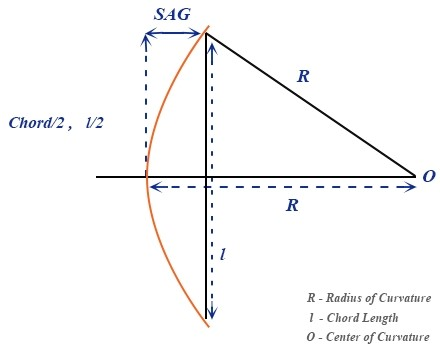
\includegraphics[width=0.48\textwidth]{Plots/radius.png}
    \caption{The construction used to calculate the radius of curvature from the length of the chord.~\cite{radius_calculator}}
    \label{fig:radius}
\end{wrapfigure}

The first thing to note in \cref{fig:positron_track} is the lead plate splitting the image in two. This plate is quoted as \SI{6}{\milli\metre} thick but the width seems to vary between the left and right side of the image. We took the left side, particularly the lighter coloured section between the thin dark lines, to be \SI{6}{\milli\metre} thick and based all of our scaling on this measurement. Not shown in this image given in \cite{Pos_Electron} is the magnetic field with lines pointing into the page and with strength \SI{1.5}{\tesla}. 


We assumed that the particle entered from the bottom, passed through the plate, and exited out the top. This was based on the fact that, provided the two tracks belong to the same particle, the lower track clearly has a larger radius of curvature, thus has a higher energy and it is nonsensical to think the particle gained energy as it passed through the lead. We were then able to find the radius of curvature for both tracks and, using \cref{eqn:radius}, find the momentum for each track. This of course requires knowing the charge of the particle, which we kindly borrow from \cite{Pos_Electron} as being the same as the proton. 


Finding the radius of the track was done with a simple graphical method, printing out the picture and using the construction in \cref{fig:radius}. It can easily be seen that $R=\frac{\mathrm{SAG}^2+\left(\frac{l}{2}\right)^2}{2\;\mathrm{SAG}}$. 

The mass stopping power was the last to be calculated. This was found by finding the difference in momentum between tracks (taking momentum equal to energy), dividing that by the distance travelled ($\approx \SI{6}{\milli\metre}$), and then dividing by the density of lead. 

\begin{figure}[h]
    \begin{center}
        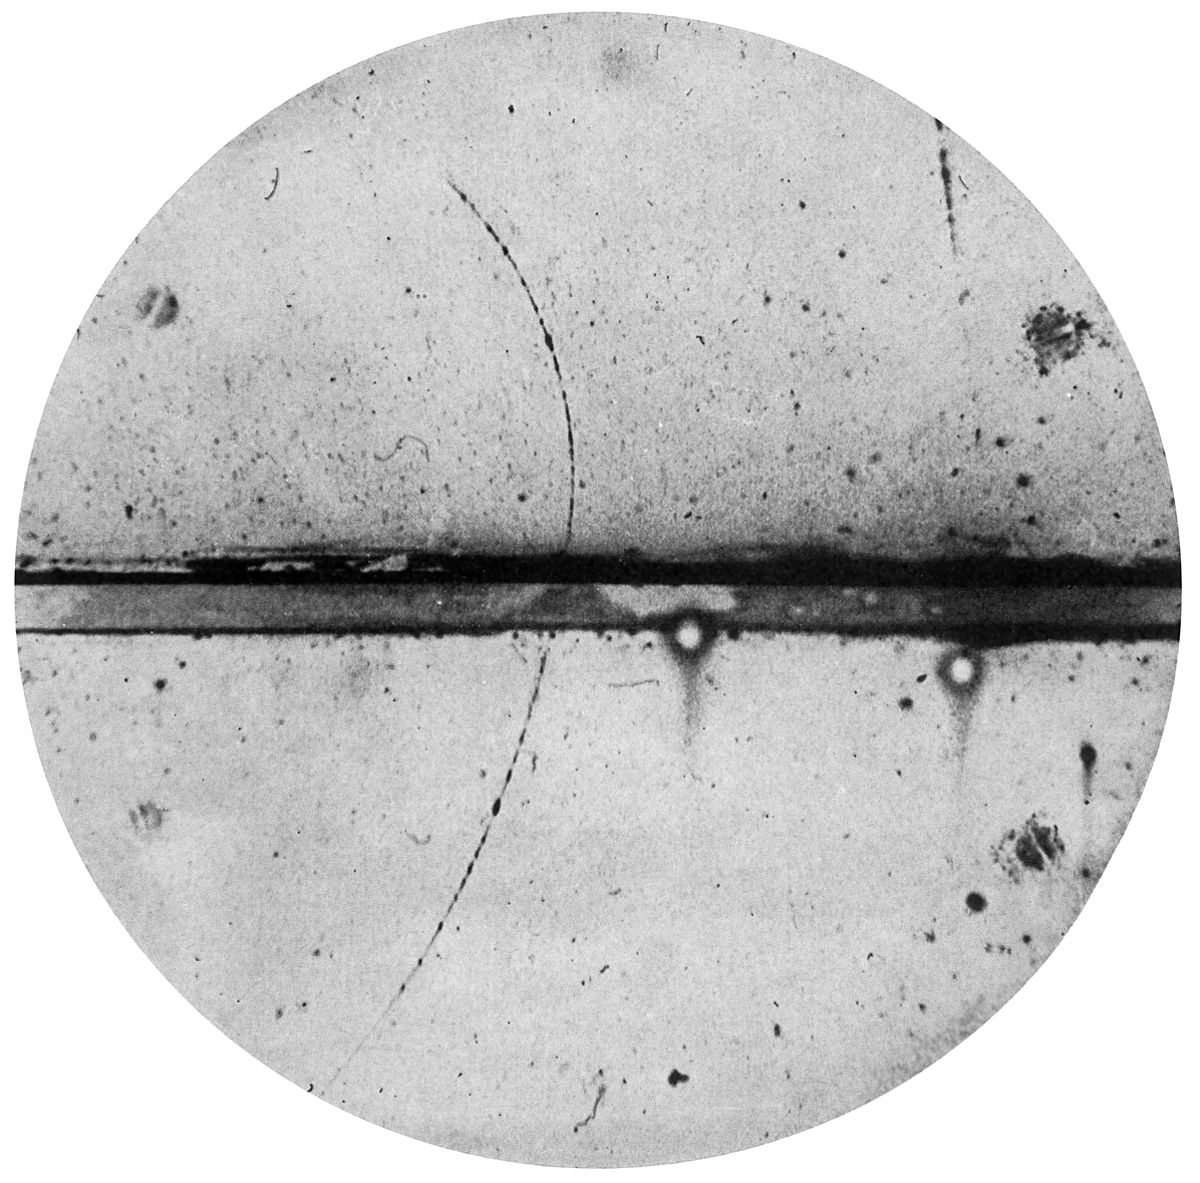
\includegraphics[width=.5\textwidth]{Plots/positron_track.jpg}
        \caption{A photograph of a particle track in a cloud chamber. A \SI{6}{\milli\metre} plate of lead separates the top and bottom halves of the image and the particle track clearly intersects this plate. A magnetic field of \SI{1.5}{\tesla} is applied uniformly, pointing into the page. \cite{Pos_Electron}}
        \label{fig:positron_track}
    \end{center}
\end{figure}


\section{Results}\label{sec:Results}
The radii and momenta of the tracks are shown in \cref{tbl:results}

\begin{table}[H]
    \centering
    \begin{tabular}{c||c|c}
         & Radius (\si[]{\milli\metre}) & Momentum (\si[]{\mega\electronvolt\per c})\\ \hline
        Incoming: & \num{128.1\pm4.7} & \num{57.6\pm2.1} \\
        Outgoing: & \num{51.2\pm1.2} & \num{23.02\pm0.54}
    \end{tabular}
    \caption{Radii and momenta of the incoming and outgoing tracks.}
    \label{tbl:results}
\end{table}

The mass stopping power for the positron in lead was found to be \SI{5.10\pm0.32}{\mega\electronvolt\centi\metre\squared\per\gram}. The electron mass stopping power for \SI{57.6\pm2.1}{\mega\electronvolt\per c} in lead is \SI{9.367}{\mega\electronvolt\centi\metre\squared\per\gram}~\cite{NIST_ESTAR}(uncertainty not specified). 

\section{Discussion}\label{sec:Discussion}
Here is the best place to discuss some of the decisions made in conducting this analysis. We used \cite{Pos_Electron} to give us some information about the particle. They decide that the particle must have charge with magnitude equal to the electron and we take this assumption at face value as we do not have the tools to deduce this. 

The sign of the charge was determined by knowing that the particle entered the chamber from the bottom and curved to the left, as discussed in \cref{sec:Method}, and knowing that the magnetic field lines pointed into the page. Simply using the right hand rule we could see that the particle had to have positive charge in order to have that trajectory. From there, we were able to find the momentum of the particle in the two regions using the graphical method. 

We were unable to determine mass and so the determination of energy for each track is impossible, but we could still determine energy loss. The mass stopping power was found to be about half that expected from the electron, which most likely speaks to the inherent inaccuracies associated with the assumptions made in the analysis, namely the fact that we assumed the particle was travelling perfectly in the plane of the image, leading to inaccurate measurements of momenta and energy loss.

\section{Conclusion}\label{sec:Conclusion}
We used a graphical method to determine the radius of curvature for two tracks in the cloud chamber image \cref{fig:positron_track} and using \cref{eqn:radius} found the momentum of the particle in the two regions, shown in \cref{tbl:results}. We assumed the particle travelled in the plane of the image only and used the determination of the charge magnitude from the original paper by Anderson.

The mass stopping power was found to be about half that of the expected value for an electron of the same energy, at \SI{5.10\pm0.32}{\mega\electronvolt\centi\metre\squared\per\gram}, which could be explained by the simplifications needed to perform the analysis, as well as inaccuracy in the image itself (the thickness of the plate being ambiguous). 

\newpage
\printbibliography


\end{document}